\section{Evaluation of Category Mapping}
We implemented two different approaches for mapping the Wikipedia article titles to the IAB taxonomy. The first approach was to create a mapping between Wikipedia categories and a describing category in the IAB taxonomy based on matching of words. The other approach was to create a mapping between excerpts of full paths and their most describing IAB category.

\subsubsection{Mapping from Wikipedia Categories to Output Categories}
Creating a mapping between Wikipedia categories and the IAB taxonomy was found to be difficult. The mapping was based on the matching words in the Wikipedia category with words in the IAB taxonomy, and only equal words were considered a match. A perfect result for such an approach is only achievable if the computer is able to understand natural language, i.e., know all synonyms, inflections and the true meaning of all words. There exists many projects for natural language processing, the most common is probably WordNet \cite{wordnet}, which shows that this task is a lot larger than the scope of our project. 

The other encountered with the mapping was ambiguous words in the category names. Figure \ref{fig:ambiguous_category_name} shows two categories that both contain the word \emph{Cicero}, but where the first category is for the suburb of Illinois \cite{wiki:ciceroillinois} and the other is for the Roman philosopher \cite{wiki:ciceroroman}. Creating mapping rules for these names would be a difficult or even impossible task. 

\begin{figure}[h]
\centering
\begin{lstlisting}
Category:Cicero, Illinois
Category:Cicero
\end{lstlisting}
\caption[Similar category names with different meaning]{Example of two category names which contains the same word with different meaning, and should be classified to different categories.}
\label{fig:ambiguous_category_name}
\end{figure}


The conclusion for this approach is that it might be possible to create a mapping from a Wikipedia category to one or more desirable output categories, but this would need a very specified third tier in the IAB category and lots of rules. The task would therefore resemble a manual classification and is not a desirable approach. 
%-> It is impossible to create a third tier to satisfy this. 

\subsection{Mapping from Path Excerpts to Output Categories}
Mapping between excerpts of Wikipedia category paths and IAB categories has the advantage that we can avoid ambiguity even though the category name is ambiguous. This approach is based on mapping rules between path excerpts and IAB categories. Manually creating these mapping rules  is still a tedious process. Thus, it is desirable to make the process as automatic as possible, which led to an automatic approach.

\subsubsection{Automatic mapping from path excerpts to output categories}
We started out by manually creating mappings between path excerpts and IAB categories, but this is a large task since there exists so many categories and category links in Wikipedia's structure. Thus, we tried to find a good way to predict matches between the excerpts and the output categories. We assumed that the IAB subcategory name (i.e., \emph{Auto parts}) is a category, and wanted to find the most likely categories leading to this category. This was done by finding all categories leading to this category among the top 3 category paths for each Wikipedia title, and counting the occurrences. The top 10 categories for each IAB subcategory was printed, and we kept all categories which occurred often. 

An evaluation was needed to see if the automated categorization process was successful. We decided to evaluate the automatic results for the subcategories of \emph{Automotive} with a manual classification for the same categories. Figure \ref{fig:manualclassification} is the results of the manual categorization of \emph{Automotive}, while figure \ref{fig:autoclassification1}, figure \ref{fig:autoclassification2} and figure \ref{fig:autoclassification3} represents the top 10 results automatically found for each of \emph{Automotive}'s subcategories.

%these results had to be compared to a manual categorization. We tested the automated categorization process on the category \emph{Automotive}. 

\begin{figure}[h]
\centering
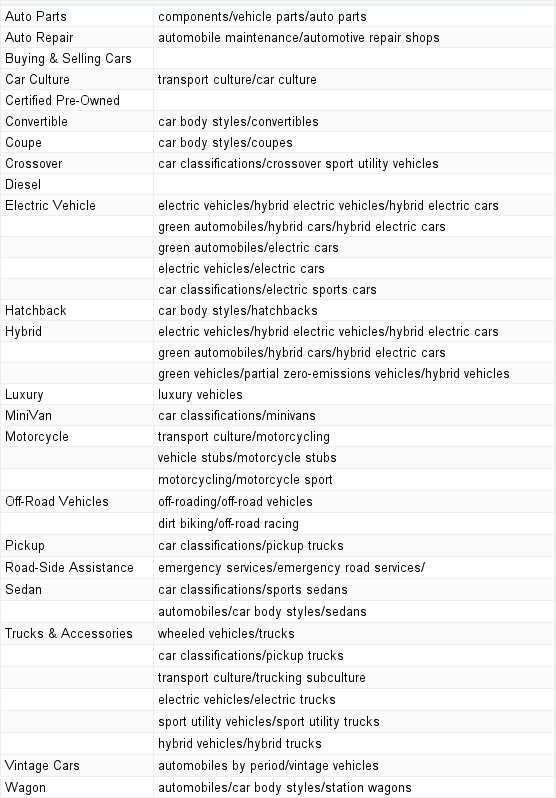
\includegraphics[width=\textwidth]{Chapters/Results/Manual_classification}
\caption[Manually mapping between categories and path excerpts]{Manually finding path excerpts for the mapping process to subcategories of \emph{Automotive}.}
\label{fig:manualclassification}
\end{figure}

\begin{figure}
\centering
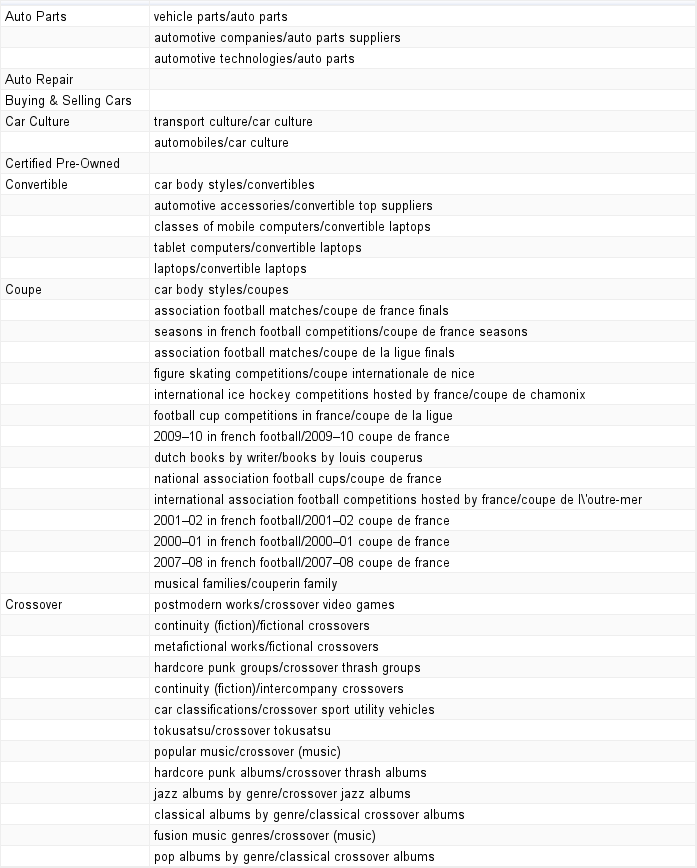
\includegraphics[width=\textwidth]{Chapters/Results/Automatic_classification_1}
\caption[Automatic mapping between categories and path excerpts, part 1]{Automatically finding path excerpts for the mapping process to subcategories of \emph{Automotive} (part 1).}
\label{fig:autoclassification1}
\end{figure}


\begin{figure}[h]
\centering
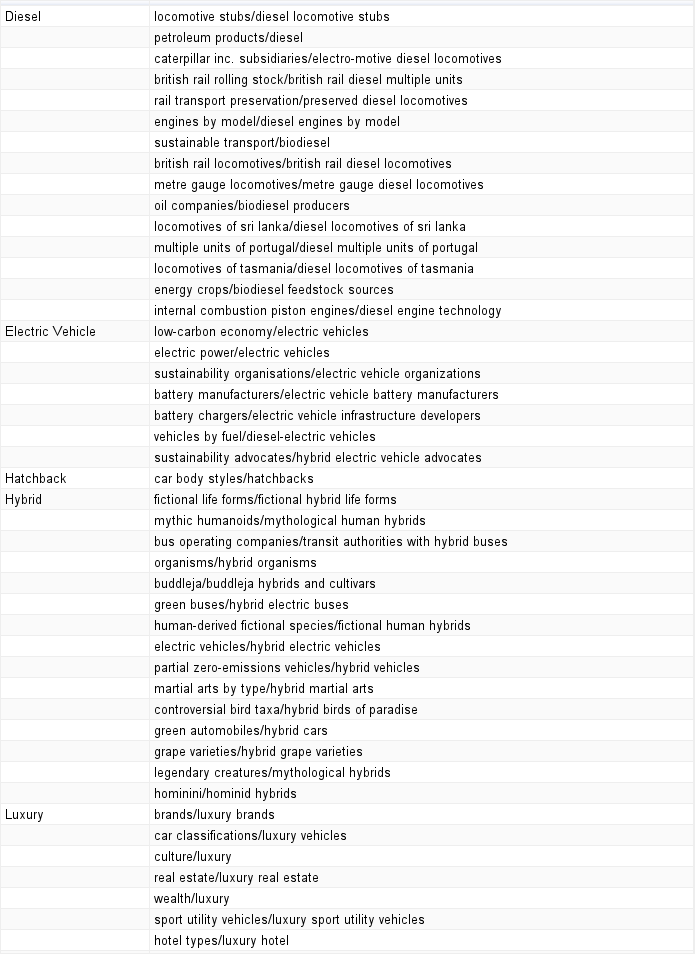
\includegraphics[width=\textwidth]{Chapters/Results/Automatic_classification_2}
\caption[Automatic mapping between categories and path excerpts, part 2]{Automatically finding path excerpts for the mapping process to subcategories of \emph{Automotive} (part 2).}
\label{fig:autoclassification2}
\end{figure}



\begin{figure}[h]
\centering
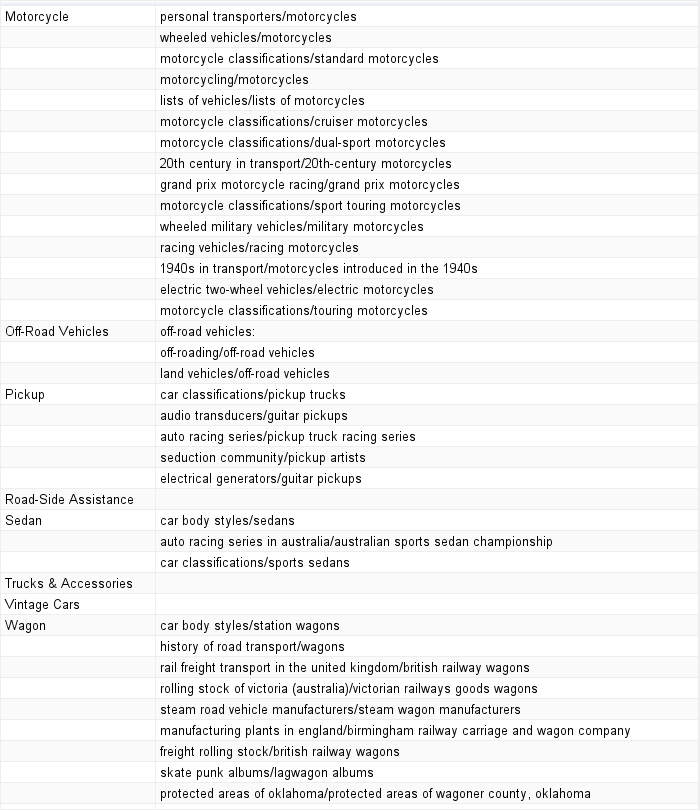
\includegraphics[width=\textwidth]{Chapters/Results/Automatic_classification_3}
\caption[Automatic mapping between categories and path excerpts, part 3]{Automatically finding path excerpts for the mapping process to subcategories of \emph{Automotive} (part 3).}
\label{fig:autoclassification3}
\end{figure}

Figure \ref{fig:wrong_automatic} illustrates a path excerpts that is not correct, which most humans will understand by common knowledge, while the computer needs lots of additional knowledge for being able to understand the same. Thus, some heuristics and human validation were needed to improve the results of the automatic categorization. 

\begin{figure}[h]
\centering
\begin{lstlisting}
Coupe:
2001-02 in french football/2001-02 coupe de france
\end{lstlisting}
\caption{Example of automatic categorization that does not work.}
\label{fig:wrong_automatic}
\end{figure}

After applying human validation, the results for \emph{Automotive} were fond in figure \ref{fig:finalclassification1} and figure \ref{fig:finalclassification2}. These results can be viewed as giving common knowledge  to the classifier, so that it is able to find patterns within the paths for categorization. Figure \ref{fig:number_of_path_excerpts_automotive} shows number of paths found for each of subcategories of Automotive, where we can see that the final results contains a higher number of path excerpts than the manual mapping, but a lower number than the automatic approach where some of the paths were removed since they were not considered relevant when validated manually.

\begin{figure}[h]
\centering
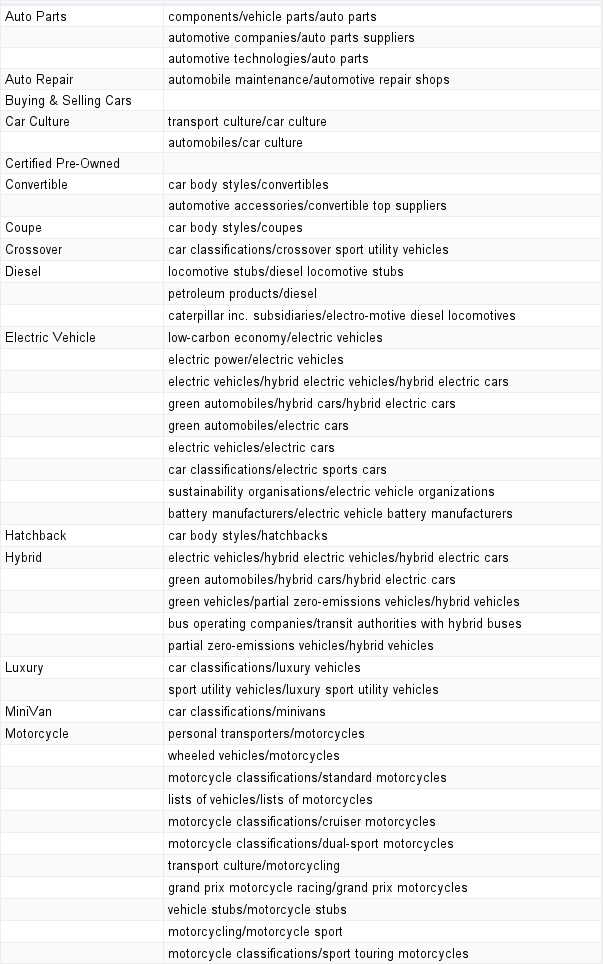
\includegraphics[width=\textwidth]{Chapters/Results/Final_classification_1}
\caption[Final results of mapping between path excerpts and IAB, part 1]{Final results of the path excerpts leading to each of \emph{Automotive}'s subcategories (part 1).}
\label{fig:finalclassification1}
\end{figure}


\begin{figure}[h]
\centering
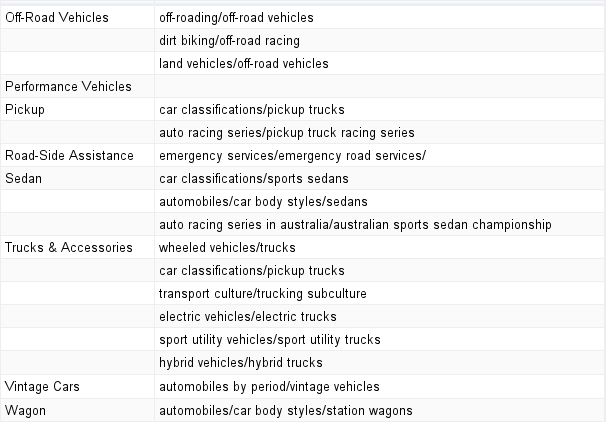
\includegraphics[width=\textwidth]{Chapters/Results/Final_classification_2}
\caption[Final results of mapping between path excerpts and IAB, part 2]{Final results of the path excerpts leading to each of \emph{Automotive}'s subcategories (part 2).}
\label{fig:finalclassification2}
\end{figure}

\begin{figure}[h]
\centering
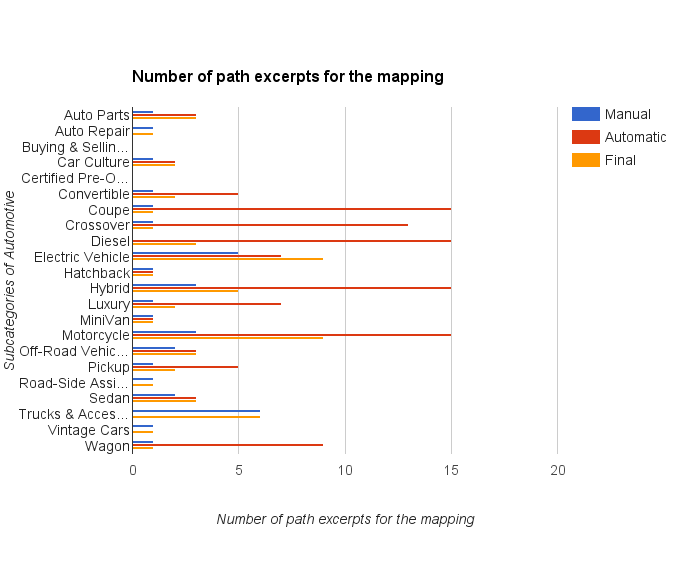
\includegraphics[width=\textwidth]{Chapters/Results/Number_of_path_excerpts_automotive}
\caption{Number of paths found for each of subcategories of Automotive. }
\label{fig:number_of_path_excerpts_automotive}
\end{figure}

\begin{comment}

Our conclusion was that it was still necessary to 

Our mapping process between path excerpts of Wikipedia categories and IAB categories has to be controlled by humans. It is desirable to make this task as automatic as possible. 

The mapping process is not completely automated since the mapping between path excerpts of Wikipedia categories and IAB categories has to be evaluated by humans. 



INSERT EXAMPLE ABOUT WALKING HERE. 
%\end{comment}

There are two main problems with manual mapping between excerpts from article paths and categories. The first problem is that the process is difficult and takes lots of time

One of the main reasons for making it an automatic process is that the process easily can be created into a 


Manually mapping between excerpts of article paths and categories is a tedious process. It is desirable to make this  process automatic or close to automatic. The reason for this is so that it is easy to create 



-automobiles/car body styles/station wagons


Eksempel på hvor variert de ulike pathene kan bli
coltainville:
* 8.72045433333 geography/geography stubs/europe geography stubs/france geography stubs/centre (region) geography stubs/eure-et-loir geography stubs/
* 8.81607333333 sports/physical exercise/dance/choreography/narratology/genres/non-fiction/non-fiction literature/historical documents/political charters/constitutions/forms of government/republics/france/geography of france/france geography stubs/centre (region) geography stubs/eure-et-loir geography stubs/
* 8.82085425    culture/cultural spheres of influence/romance countries and territories/france/geography of france/france geography stubs/centre (region) geography stubs/eure-et-loir geography stubs/


Alle:
[INFO] Total number of articles found: 152 664/4690240
[INFO] books & literature: 189169 articles



Kun 6 kategorier etter: 33 104/4690240
[INFO] books & literature: 51919 articles

-> len(cats_at_end) > 5: 

Kun 4 kategorier etter: 



\end{comment}